
% ----------------------------------------------------------------------
%                   LATEX TEMPLATE FOR PhD THESIS
% ----------------------------------------------------------------------

% based on Harish Bhanderi's PhD/MPhil template, then Uni Cambridge
% http://www-h.eng.cam.ac.uk/help/tpl/textprocessing/ThesisStyle/
% corrected and extended in 2007 by Jakob Suckale, then MPI-CBG PhD programme
% and made available through OpenWetWare.org - the free biology wiki


%: Style file for Latex
% Most style definitions are in the external file PhDthesisPSnPDF.
% In this template package, it can be found in ./Latex/Classes/
\documentclass[twoside,11pt]{Latex/Classes/PhDthesisPSnPDF}


%: Macro file for Latex
% Macros help you summarise frequently repeated Latex commands.
% Here, they are placed in an external file /Latex/Macros/MacroFile1.tex
% An macro that you may use frequently is the figuremacro (see introduction.tex)
% % This file contains macros that can be called up from connected TeX files
% It helps to summarise repeated code, e.g. figure insertion (see below).

% insert a centered figure with caption and description
% parameters 1:filename, 2:title, 3:description and label
\newcommand{\figuremacro}[3]{
	\begin{figure}[htbp]
		\centering
		\includegraphics[width=1\textwidth]{#1}
		\caption[#2]{\textbf{#2} - #3}
		\label{#1}
	\end{figure}
}

% insert a centered figure with caption and description AND WIDTH
% parameters 1:filename, 2:title, 3:description and label, 4: textwidth
% textwidth 1 means as text, 0.5 means half the width of the text
\newcommand{\figuremacroW}[4]{
	\begin{figure}[htbp]
		\centering
		\includegraphics[width=#4\textwidth]{#1}
		\caption[#2]{\textbf{#2} - #3}
		\label{#1}
	\end{figure}
}

% inserts a figure with wrapped around text; only suitable for NARROW figs
% o is for outside on a double paged document; others: l, r, i(inside)
% text and figure will each be half of the document width
% note: long captions often crash with adjacent content; take care
% in general: above 2 macro produce more reliable layout
\newcommand{\figuremacroN}[3]{
	\begin{wrapfigure}{o}{0.5\textwidth}
		\centering
		\includegraphics[width=0.48\textwidth]{#1}
		\caption[#2]{{\small\textbf{#2} - #3}}
		\label{#1}
	\end{wrapfigure}
}

% predefined commands by Harish
\newcommand{\PdfPsText}[2]{
  \ifpdf
     #1
  \else
     #2
  \fi
}

\newcommand{\IncludeGraphicsH}[3]{
  \PdfPsText{\includegraphics[height=#2]{#1}}{\includegraphics[bb = #3, height=#2]{#1}}
}

\newcommand{\IncludeGraphicsW}[3]{
  \PdfPsText{\includegraphics[width=#2]{#1}}{\includegraphics[bb = #3, width=#2]{#1}}
}

\newcommand{\InsertFig}[3]{
  \begin{figure}[!htbp]
    \begin{center}
      \leavevmode
      #1
      \caption{#2}
      \label{#3}
    \end{center}
  \end{figure}
}


%%% Local Variables: 
%%% mode: latex
%%% TeX-master: "~/Documents/LaTeX/CUEDThesisPSnPDF/thesis"
%%% End: 

\usepackage[T1]{fontenc}
\usepackage{array}
\usepackage{pdfpages}
\usepackage{xspace}
\usepackage{xcolor}
\usepackage{lipsum}
\usepackage{makecell}
\usepackage{tabularray}
\usepackage{xcolor}
\usepackage{longtable}

%\usepackage{graphics}
% or use the graphicx package for more complicated commands
%\usepackage{graphicx}

%: ----------------------------------------------------------------------
%:                  TITLE PAGE: name, degree,..
% ----------------------------------------------------------------------
\usepackage{graphicx}

      \textwidth 15cm
      \textheight 22cm
      \parindent 10pt
      \oddsidemargin 0.85cm
      \evensidemargin 0.37cm
     
\newcommand{\ie}{\emph{i.e.,}\xspace}
\newcommand{\eg}{\emph{e.g.,}\xspace}
\newcommand{\etc}{etc.\xspace}
\newcommand{\etal}{\emph{et~al.}\xspace} 

\newcommand{\todo}[1]{\textcolor{blue}{#1}} 

\begin{document}

\thispagestyle{empty}

\begin{center}

Vrije Universiteit Amsterdam 

\vspace{1mm}


\includegraphics[height=20mm]{0_frontmatter/figures/vu-griffioen.pdf}

\vspace{2cm}

{\Large Master Thesis}

\vspace*{1.5cm}

\rule{.9\linewidth}{.6pt}\\[0.4cm]
{\huge \bfseries Enforcing citizens' privacy with information technology\par}\vspace{0.4cm}
\rule{.9\linewidth}{.6pt}\\[1.5cm]

\vspace*{2mm}

{\Large
\begin{tabular}{l}
{\bf Author:} Maarten Swaap (Student number 2644292)
\end{tabular}
}

\vspace*{2cm}

\begin{tabular}{ll}
{\it 1st supervisor:}   & ~~prof. dr. Patricia Lago \\
%{\it daily supervisor:} & ~~dr. Michiel van der Veen (Director Innovation and Development,\\ & ~~National Office for Identity Data) \\
{\it 2nd reader:}       & ~~Roberto Verdecchia %or dr. Remco de Boer 
\end{tabular}

\vspace*{2.5cm}

\textit{A thesis submitted in fulfillment of the requirements for\\ the VU Master of Science degree in Information Science}

\vspace*{1.8cm}

\today\\[4cm] % Date

\end{center}

\newpage


% ----------------------------------------------------------------------
       
% turn of those nasty overfull and underfull hboxes
\hbadness=10000
\hfuzz=50pt


%: --------------------------------------------------------------
%:                  FRONT MATTER: dedications, abstract,..
% --------------------------------------------------------------


%\language{english}


% sets line spacing
\renewcommand\baselinestretch{1.2}
\baselineskip=18pt plus1pt


%: ----------------------- generate cover page ------------------------

\begin{center}
\textit{Architectural patterns and tactics to mitigate identity fraud}
\end{center}

%: ----------------------- cover page back side ------------------------
% Your research institution may require reviewer names, etc.
% This cover back side is required by Dresden Med Fac; uncomment if needed.

\newpage
%\vspace{10mm}
%1. First Reader: Name Surname
%
%\vspace{10mm}
%2. Daily Supervisor: Name Surname
%
%\vspace{10mm}
%3. Second Reader: Name Surname
%
%\vspace{10mm}
%4. Industrial Supervisor: Name Surname
%
%\vspace{20mm}
%Day of the defense:

%\vspace{20mm}
%\hspace{70mm}Signature from head of PhD committee:



%: ----------------------- abstract ------------------------

% Your institution may have specific regulations if you need an abstract and where it is to be placed in the document. The default here is just after title.


% Thesis Abstract -----------------------------------------------------


%\begin{abstractslong}    %uncommenting this line, gives a different abstract heading
\begin{abstracts}        %this creates the heading for the abstract page

\noindent \textit{Context}. 
Privacy of citizens is protected by law. However, leakage of citizens' data occurs more often with possible impact on the live of these citizens.

\noindent \textit{Goal}. 
Goal of this research is to provide an overview of the domain of identity theft and to provide a definition of concrete problems together with possible solutions.

\noindent \textit{Method}. 
Research experiment has been executed based on literature study and semi-structured interviews with experts in the field of identity data within the government. 
Using coding to extract information from the semi-structured interviews.

\noindent \textit{Results}. 
The extracted Business Goals and Concerns resulted in Architectural Significant requirements which lead to possible privacy mitigating solutions as examples for implementation.

\noindent \textit{Conclusions}. 
Identity theft is a broad domain and to solve problems it needs scoping. In the solution part Architectural Significant Requirements can facilitate in selecting an appropriate solution.

\end{abstracts}
%\end{abstractlongs}


% ---------------------------------------------------------------------- 


% The original template provides and abstract separate environment, if your institution requires them to be separate. I think it's easier to print the abstract from the complete thesis by restricting printing to the relevant page.
% \begin{abstractseparate}
%   
% Thesis Abstract -----------------------------------------------------


%\begin{abstractslong}    %uncommenting this line, gives a different abstract heading
\begin{abstracts}        %this creates the heading for the abstract page

\noindent \textit{Context}. 
Privacy of citizens is protected by law. However, leakage of citizens' data occurs more often with possible impact on the live of these citizens.

\noindent \textit{Goal}. 
Goal of this research is to provide an overview of the domain of identity theft and to provide a definition of concrete problems together with possible solutions.

\noindent \textit{Method}. 
Research experiment has been executed based on literature study and semi-structured interviews with experts in the field of identity data within the government. 
Using coding to extract information from the semi-structured interviews.

\noindent \textit{Results}. 
The extracted Business Goals and Concerns resulted in Architectural Significant requirements which lead to possible privacy mitigating solutions as examples for implementation.

\noindent \textit{Conclusions}. 
Identity theft is a broad domain and to solve problems it needs scoping. In the solution part Architectural Significant Requirements can facilitate in selecting an appropriate solution.

\end{abstracts}
%\end{abstractlongs}


% ---------------------------------------------------------------------- 

% \end{abstractseparate}


%: ----------------------- tie in front matter ------------------------

\frontmatter
% Thesis Dedication ---------------------------------------------------

%\begin{dedication} %this creates the heading for the dedication page

%To ...

%\end{dedication}

% ----------------------------------------------------------------------
% Thesis Acknowledgements ------------------------------------------------


%\begin{acknowledgementslong} %uncommenting this line, gives a different acknowledgements heading
%\begin{acknowledgements}      %this creates the heading for the acknowlegments


%\end{acknowledgements}
%\end{acknowledgmentslong}

% ------------------------------------------------------------------------





%: ----------------------- contents ------------------------

\setcounter{secnumdepth}{3} % organisational level that receives a numbers
\setcounter{tocdepth}{3}    % print table of contents for level 3
\tableofcontents            % print the table of contents
% levels are: 0 - chapter, 1 - section, 2 - subsection, 3 - subsection


%: ----------------------- list of figures/tables ------------------------

\listoffigures	% print list of figures
\listoftables  % print list of tables

%: ----------------------- glossary ------------------------

% Tie in external source file for definitions: /0_frontmatter/glossary.tex
% Glossary entries can also be defined in the main text. See glossary.tex
% 
%% this file is called up by thesis.tex
% content in this file will be fed into the main document

% Glossary entries are defined with the command \nomenclature{1}{2}
% 1 = Entry name, e.g. abbreviation; 2 = Explanation
% You can place all explanations in this separate file or declare them in the middle of the text. Either way they will be collected in the glossary.

% required to print nomenclature name to page header
%\markboth{\MakeUppercase{\nomname}}{\MakeUppercase{\nomname}}


% ----------------------- contents from here ------------------------


%\nomenclature{LSY}{ehbfuefebbfbjkjkebfjbfbfw} 
%\nomenclature{DEPC}{diethyl-pyro-carbonate; used to remove RNA-degrading enzymes (RNAases) from water and laboratory utensils}
%\nomenclature{DMSO}{dimethyl sulfoxide; organic solvent, readily passes through skin, cryoprotectant in cell culture}
%\nomenclature{EDTA}{Ethylene-diamine-tetraacetic acid; a chelating (two-pronged) molecule used to sequester most divalent (or trivalent) metal ions, such as calcium (Ca$^{2+}$) and magnesium (Mg$^{2+}$), copper (Cu$^{2+}$), or iron (Fe$^{2+}$ / Fe$^{3+}$)}



 

%\begin{multicols}{2} % \begin{multicols}{#columns}[header text][space]
%\begin{footnotesize} % scriptsize(7) < footnotesize(8) < small (9) < normal (10)

%\printnomenclature[1.5cm] % [] = distance between entry and description
%\label{nom} % target name for links to glossary

%\end{footnotesize}
%\end{multicols}



%: --------------------------------------------------------------
%:                  MAIN DOCUMENT SECTION
% --------------------------------------------------------------

% the main text starts here with the introduction, 1st chapter,...
\mainmatter

\renewcommand{\chaptername}{} % uncomment to print only "1" not "Chapter 1"


%: ----------------------- subdocuments ------------------------

% Parts of the thesis are included below. Rename the files as required.
% But take care that the paths match. You can also change the order of appearance by moving the include commands.

\chapter{Introduction}\label{s:intro}

%\todo{
%This section includes some motivations behind the work, explicitly or implicitly
%highlights the research question, provides a high-level explanation of the
%solution, and describes the contributions.}

\section{Motivation}
The main objective of this research is scoping the problem of identity theft to make it possible to decompose the problem to quality attributes of the ISO 25010 standard \cite{ISO:25010:2011} to support the matching process of generically usable patterns and tactics which can be applied building software.

\section{Research question}
How can information systems reduce the possibility to commit identity fraud, without losing the benefit of exchanging personal data of a citizen within the government of The Netherlands, and how can further suitability of these methods be assessed?

\begin{quote}\emph{RQ1: What is the definition of identity fraud, and which concrete problems can be identified?}\end{quote}
\begin{quote}\emph{RQ2: Which requirements are significantly relevant to assess technical suitability, and which trade offs apply between these requirements within different solutions, for broader usage within the Dutch government?}\end{quote}
\begin{quote}\emph{RQ3: Which available architectural tactics and patterns are available in order to mitigate identity fraud?}\end{quote}

\break

\section{Scientific and practical contribution of this research}
Implementing a system implies software architecture is present and architectural choices have been made. Bass '\etal \cite{Bass2015SoftwareAI} mentions the following regarding software architecture "a program or computing system is the structure or structures of the system, which comprise software elements, the externally visible properties of those elements, and the relationships among them." Also, Bass \etal claim every software system has an architecture. However, the software architecture is not always formally described.
The research objective is to identify goals and concerns relevant when designing information systems which could mitigate identity fraud. Thereafter, combining these goals and concerns in a formal description of Architecturally Significant Requirements (ASR) categorized in Quality attributes (QA) based on ISO 25010 \cite{ISO:25010:2011}. Based on these QA's and ASRs a selection of available architectural patterns and tactics will be discussed and possible trade-offs will be reasoned upon.

This will contribute in selecting the appropriate technologies to mitigate identity fraud. Making use of a selection of already existing architectural patterns and tactics which can be applied in information systems. The provided definition and quantification of identity theft can be used to raise awareness on this problem and serve as a base for future research on this topic.

Contribution to science and practice will be achieved by defining relevant quality attributes for designing information systems. Concerning the Quality attributes of the ISO 25010 standard, not only the attribute 'Security' will be taken into account. Business goals and concerns will provide a broader perspective for developing information systems. The patterns and tactics can help designers and builders build and assess their information system.

This research facilitates in examples, and not the definition, on which methods should be used for implementation. Also, it can be assumed that business goals, concerns, architecturally significant requirements and technology will evolve over time, resulting in a continuously evolving set of variables to take in account when designing or evaluating information systems.
\chapter{Background}\label{s:background}
%\todo{This section provides the necessary context to help the reader understand the remainder of the thesis.}
\section{Problem definition}
One of the main objectives of the Digitale Overheid (Digital Government) is to 'Protect fundamental rights and public values'\cite{DO_agenda}. One could argue protecting the identity and privacy of citizens is part of this objective.The objective of this research is to help reduce the opportunity of identity theft and simultaneously improve citizens’ privacy by making use of appropriate information systems.


\subsection{Researching and defining the specific problem and objective}
The Unique Identity Number (UIN) of the Dutch citizen is the ‘Burger Service Nummer’, abbreviated by BSN (English: ‘Citizen Service Number’). It’s comparable with the Social Security Number in the USA, but it is also being used for different purposes in The Netherlands. \par
The Dutch governmental audit service, Auditdienst Rijk (ADR) defined gaps and possible improvements in usage of this number\cite{ADR}. In this report the big advantage of BSN is concluded to be a unique identifier for many different government and non-government organizations. Making their administration done more easily. On the other hand, another main objective by introducing BSN was to prevent identity fraud. Facts and figures in the report of ADR are showing Identity Fraud is becoming a bigger issue. The problem for citizens is that using the BSN could impact the privacy of citizens negatively, while having great benefits for the Dutch government. The same BSN is re-used for different purposes. For example, a bank uses the same BSN of a citizen as a hospital. If the hospital would have a data breach, the BSN could be re-used when committing identity fraud, for example at a bank. However, the solely having the BSN makes identity fraud difficult. 
Firstly, during this research it became clear that a UIN is only a part of the problem. Secondly, a clear definition of identity theft is needed to prevent different viewpoints of the problem when discussing solutions. Also, quantifying and scoping on a part of the problem will help in discussing possible and appropriate information systems.
\par

\section{Scope}
To position problem and solution correctly, it is needed to define and scope definition and problem within this research. A UIN is part of a persons Identity data. But it's only one element within the identity data connected to an individual person. Thus, it's important to frame the position of a UIN among with other data within in this domain.
De Vries \etal \cite{Vries2007IdentiteitsfraudeEA} split up 'Means of identification' (for example a passport or drivers licence) and 'Identity data' for analytical purposes. This research will focus on 'Identity data'. It cannot be denied identity fraud applies on both domains, but because of restrictions in time and resources focus is needed. 

\subsection{Description of identity data types} \label{Identity_datatypes}
Figure \ref{fig:ID_domain} decomposes the domain described by De Vries \etal. This research is scoped at 'Formal functional identity data'. In certain way 'Profile data' has overlap with this research, because a UIN can be used in facilitating combination of data-sets and unauthorized profiling. Definitions provided by De Vries \etal: 
\graphicspath{ {./images/} }
\begin{figure}[t]
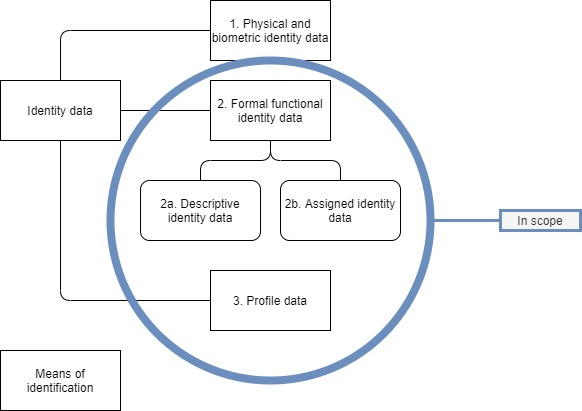
\includegraphics[width=10cm]{Identity data defintions and domain-Overview.jpg}\\
\caption{Domain of Identity Data.}
\label{fig:ID_domain}
\end{figure}
\begin{enumerate}
\item \textit{Physical and bio-metric identity data} - General physically identification data. For example, sex, height, hair color, iris, DNA-profile or medical history
\item \textit{Formal functional identity data} - Data assigned or ascribed in a certain stage of phase of life. To functionally distinguish individuals and assign rights and obligations to this individual.
\begin{enumerate}
\item \textit{Descriptive identity data} - Data that describes a person and the persons surroundings. Information that is close to the individual and is factual and mostly static. For example, family-name, parents, Place, date and time of birth. 
\item \textit{Assigned identity data} - Data that is assigned and mostly describes a (contractual) relationship with organisations to provide products and services.
\end{enumerate}
\item \textit{Profile data} - Based on a certain set of factual data, an algorithm defines profiles that categorize a person. 
\end{enumerate}

\subsection{Definition of Identity Fraud - scoped at Identity theft for this research}
While executing this research it became clear that identity Fraud is a catch-all term. De Vries \etal \cite{97408536fd1c4f4e9d1615b7a4a4473e} have analysed 30 international definitions and formulated a general description "Identity Fraud is to obtain, to possess or to create intentionally, (and) (unlawfully or without consent) false means of identification
in order to commit unlawful behaviour, or to have the intention to commit unlawful behaviour." In the footnote it states: "It must be noted that ‘false’ in the description refers to the idea that the means of identification do not identify the person who uses them truthfully." It's needed to say this is a generic definition. Figure \ref{fig:ID_fraud} shows the different types of mismatch between a person and identity data, defined by De Vries \etal \cite{Vries2007IdentiteitsfraudeEA}. This research will focus on a subset of Identity Fraud, namely Identity Theft.
\graphicspath{ {./images/} }
\begin{figure}[t]
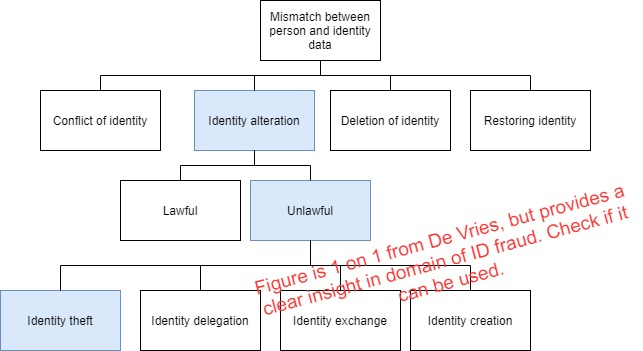
\includegraphics[width=10cm]{Domain of Identity fraud.jpg}\\
\caption{Domain of Identity Fraud}
\label{fig:ID_fraud}
\end{figure}

\subsection{Quantitative impact of Identity Fraud}\label{Quantitative_impact}
De Vries \etal state it's difficult to quantify identity fraud, because it's incorporated in other crimes.\cite{Vries2007IdentiteitsfraudeEA}. Goudriaan \etal claim many crimes in Western countries are not even reported to the police \cite{Gourdriaan_etal}. Quantification is relevant to define how vast a problem is and how a possible solution could mitigate it. Emphasis of this research will be logical reasoning and argumentation and not quantification of the effect of a solution. Firstly, because this is not realistic due to time restrictions. Secondly, it's needed to define an exact quantification method. Which is not the scope of this research. However, even if quantified correctly, selected countermeasures would only contain substantiated arguments by means of logical reasoning or extensive research after applying it.

A report of the Auditdienst Rijk (ADR)\cite{ADR} takes in account numbers of the citizen service for Identity Fraud at the National Office for Identity Data (Rijksdienst voor Identiteitsgegevens). Somewhere around 4.0000 citizens a year contact this service to report identity fraud. In some cases, the impact is low and only a discomfort. In other cases, the fraud results in identity theft that can lead, for example, to debts or fines.\par

However, over time Statistics Netherlands (CBS) quantified data of identity fraud, based on statistical data. Purely looking at the data classified by Identity Fraud, CBS defines it: "Without permission, via internet, making usage of someones personal data for financial gain, for example by withdraw or transfer of money, take out a loan or request of official documents." Roughly 0.5\% of Dutch citizens in 2019 became victim of identity fraud. Based on a population of 17 million, this means roughly 86.000 people are confronted with Identity Fraud each year. 
{\todo{TABEL HIER https://opendata.cbs.nl/#/CBS/nl/dataset/82464NED/table?ts=1637054627124
https://opendata.cbs.nl/#/CBS/nl/dataset/82464NED/barh?ts=1637054521497
https://opendata.cbs.nl/#/CBS/nl/dataset/82464NED/table?ts=1637054352194}}.
When looking at a broader scope, to anticipate on a definition creep, another research of the CBS is relevant {\cite{CBS_casualtiesDigitalCrime}} and zooms in on the way casualties act.

\subsection{Role of the UIN}
The World Bank \cite{WorldBank_UIN} defines ID numbers "In the context of foundational systems, ID numbers are considered to be “unique when: firstly, the number-generating process ensures that no two people within the system share the same number and secondly, a deduplication process ensures that the same person does not have multiple identity records or numbers (i.e., that they are unique in the database)." The World Bank identifies two derived strengths, namely ‘Uniqueness and deduplication’ and ‘Data matching and interoperability’. This means each person can be identified uniquely, allowing for a fast and easy exchange of identity related information between different organizations.\par 
However, the benefit of fast and easy exchange of identity related information, is also highly susceptible to misuse. Identity Fraud and Theft leans heavily on the benefit of ‘Data matching and interoperability’ of the UIN. A second form of misuse that leans on this benefit is Unauthorized data correlation. \par

\subsection{Operational problem}\label{Operational_problem}
The World Bank ID4ID defines vulnerabilities and risks when UINs are ubiquitous available \cite{WorldBank_protecting}. Identity theft and fraud and unauthorized data correlation are two operational problems. This research will focus on the practical problem of unauthorized correlation, in section \ref{Identity_datatypes} defined as 'Profile data', by using 'Formal functional identity data'. The UIN of a person can be defined as 'Assigned identity data'. Architectural patterns and tactics will focus on mitigating this problem, taking relevant QA's and ASRs into account. 
The UK national fraud and cybercrime reporting centre states only a name, date of birth and current or previous addresses is needed to commit identity fraud. \cite{Action_fraud}
Identity data can be obtained by personal data in a data breach, for example a breach via commercial parties or (semi-)government. Recent examples are Booking.com \cite{Booking_databreach} or the Dutch GGD \cite{GGD_databreach}.


\subsection{Legal implications}
\todo{replace this section for a small part on Basisregistratie personen (BRP) and exchange of identity information within government}
%Dutch laws enforce the exchange of identity data of a citizen and explicitly state to include BSN in this dataset. These laws exist in order to stimulate controlled exchange of personal data. This applies to government bodies , pension providers  and healthcare organizations. Usage of an alternative method, not explicitly providing a BSN, can be interpreted as not complying with these laws. This interpretation is not in scope for my thesis research.\par
However, technologies like encryption and pseudonymisation are explicitely stated in General Data Protection Regulation (GDPR, REGULATION (EU) 2016/679) {\cite{GDPR}} to be in place as a safeguard. Other rules and regulations may apply, but are not in scope.
%
%\subsection{Pseudonymization or tokenization of a UIN}
%Researching possible solutions in literature and consulting experts showed %two viable methods worth analyzing. Pseudonymization and tokenization. %Pseudonymization of BSN already has been applied within the Dutch %government by Logius. Previous work by AuditDienst Rijk on the usage of BSN % already discussed pseudonymization as an option. Tokenization is an %alternative method largely applied in payment sector (Adyen and Apple Pay) %to ensure privacy of customers. This method is suggested by the World Bank %as a possible solution to replace a UIN, because it’s been applied within %the governments of Austria, India and Estionia.\par
%The difference between these two techniques is mainly the method of %reversing. While pseudonymization needs a key to decrypt, the techniques %behind tokenization need a form of ledger or table to lookup the original %record.
%Off course, there are a lot more technological methods. However, the scope %of this research will not be assessing all of them, rather creating a %useful framework to assess these methods based on requirements.\par
%\textbf{Pseudonymization} 
%GDPR \cite{GDPR} defines ‘pseudonymisation’: means the processing of %personal data in such a manner that the personal data can no longer be %attributed to a specific data subject without the use of additional %information, provided that such additional information is kept separately %and is subject to technical and organisational measures to ensure that the %personal data are not attributed to an identified or identifiable natural %person; \par
%\textbf{Tokenization} is described by The World Bank  as “Tokenization can %protect privacy by ensuring that only tokens, rather than a permanent %identity number or other UIN, are exposed or stored during a transaction.” %Also, by this definition, the same person is represented by different %tokens in different databases. A fundamental property, besides it’s unique %character, is it’s not possible to reverse engineer a person’s identity, %because the unique token does not contain this data.\par
%The World Bank defines two primary types of tokenization. Firstly, %\textbf{Front-end tokenization} is the creation of a token by the user as %part of an online service that can later be used in digital transactions in %place of the original identifier value. Secondly, in case of %\textbf{Back-end tokenization} the identity provider (or token provider) %tokenizes identifiers before they are shared with other systems, limiting %the propagation of the original identifier and controlling the correlation %of data. Back-end tokenization is done automatically by the system without %user intervention, meaning that people do not need to do anything manually %or understand why they would need to create tokens, eliminating any %potential digital divide and protecting identifiers and UIN at source.”
\chapter{Overview}\label{s:overview}
\todo{check if overview matches with Implementation and covers all BG and Concerns}

This overview contains a Utility Tree, which captures the Architecturally significant requirements (ASR). These ASRs are extracted from interviews (interviewee description in Appendix  \ref{Appendix A}) and combine with the Business Goals and Concerns (available in Appendix \ref{Appendix B} and  \ref{Appendix C}) 

\graphicspath{ {./images/} }
\begin{figure}
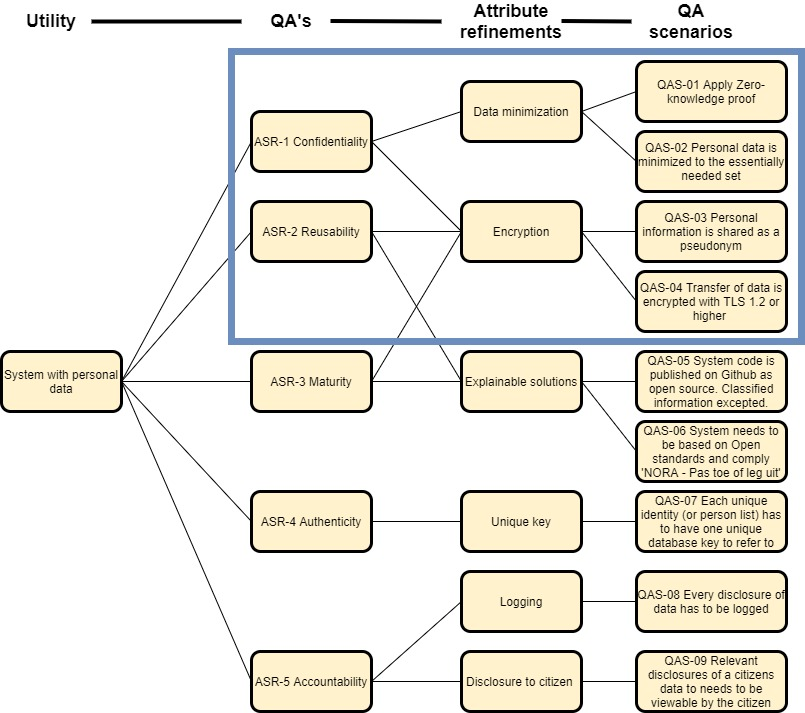
\includegraphics[width=14cm]{Decomposition of ASR and QAS-Utility Tree v3.jpg}\\
\caption{Decomposition of Architecturally significant requirements}
\label{fig:ASR1}
\end{figure}

\begin{table}[h!]
\centering
\begin{tabular}{||l l l||} 
 \hline
 Business Goal(s) (BG) & Concern(s) (C) & Architectural Significant Requirement (ASR) \\ [0.5ex] 
 \hline\hline
 \makecell {BG-03} & C-03 & ASR-1 Confidentiality \\
 \hline
 \makecell {BG-01, BG-02} & C-01, C-02 & ASR-2 Re-usability\\
\hline
 \makecell {BG-05} &  C-09 & ASR-3 Maturity  \\
 \hline
\makecell {BG-04} & C-04, C-05, C-06, C-11 & ASR-4 Authenticity \\
 \hline
 \makecell {BG-01} & C-10 & ASR-5 Accountability  \\ [1ex] 
 \hline
\end{tabular}
\caption{ASRs Plotted on business goals and concerns.}
\label{ASR_BG_C}
\end{table}

Concerns C-07, C-08 and C-11 and BG-06 are not addressed in this overview, because the scope of this research is not taking in account laws, exceptions and non-government organizations. However, these concerns are considered possible relevant for future research and therefore included in the appendix.


% \todo{
% This section provides a high-level outline of the proposed system or solution.
% It typically illustrates the system architecture or the interactions between the
% different solution components (via a “boxes-and-arrows” diagram) from a user’s
% perspective.
% }
%\chapter{Implementation}\label{s:implementation}
%\graphicspath{ {./images/} }
%\begin{figure}[t]
%\centering
%\caption{Zoomed in on QAS of ASR-1}
%\label{fig:ASR2}
%\end{figure}
%\includegraphics[width=12cm]{Decomposition of ASR and QAS_zoomed in on %ASR-1 and ASR-2_v2.jpg}\\
\chapter{Implementation}\label{s:Implementation}
Research question 3 focuses on patterns and tactics, in context of software architecture. Bass \etal \cite{Bass2015SoftwareAI} describes architectural patters as "Compositions of architectural elements and provide packaged strategies for solving some of the problems facing a system." This section contains examples of processes represented by views and contain patterns and tactics. Focusing on the quality attribute 'Confidentiality', which is the quality attribute that could mitigate the operational problems in section \ref{OP} The pattern of 'Zero-knowledge proof' and tactics of 'Data minimization' and 'Pseudonymization' mentioned by consulted experts as possible techniques to apply. By depicting different types of views on example processes, the examples are presented as possible basis for practical use. The tactics of Authentication' and 'Encryption' are more basic building blocks already applied and therefore explained more briefly.

Section \ref{QI} discusses the quantified problem and argues logical reasoning will define how a solution could mitigate the operational problem mentioned in section \ref{OP}
\section{Pattern - Zero-knowledge proof}
By definition of Goldwasser \etal \cite{Goldwasser} "A zero-knowledge proof (ZKP) makes it possible to prove a statement is true while preserving confidentiality of secret information". 
Xiaohui Yang and Wenjie Li \cite{YANG2020102050} state "Zero-knowledge proof (ZKP) is a cryptography technique, which means that the prover can convince the verifier that a certain statement is correct without providing the verifier with any additional information or leaking any information about the witness." Figure \ref{fig:ZKP_usecase} presents a schema on how this principle works. Figure \ref{fig:QAS01} presents two example Quality Attribute Scenarios (QAS) which describe desired system behaviour. The ZKProof Community reference \cite{2019:zkproof:community-reference-0.2} of Bennarroch \etal is intended to provide a reference for development of zero-knowledge proof by contribution of world-renowned cryptographers, practitioners and industry leaders.
Reasoning why this methodology or pattern is a solution for the operational problem in section \ref{OP} is if there is no identity data to be shared or replicated, there will be no profiling or unauthorized correlation of identity data can be done. Without identity data it's not possible to commit identity fraud.

\subsection{Chain of use-cases described}
\graphicspath{ {./images/} }
\begin{figure}
\centering
\label{fig:ZKP_usecase}
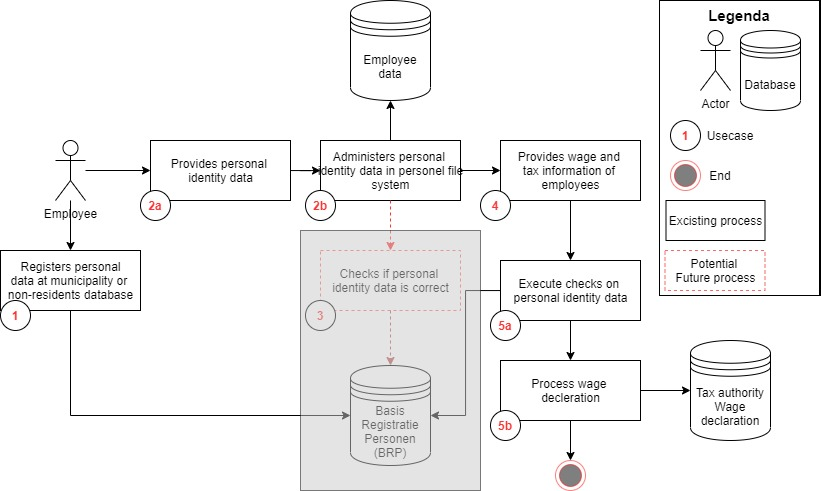
\includegraphics[width=10cm]{Usecase for zkp.jpg}\\
\caption{Scenarios - set of use-cases on one of ZKP could be applied}
\end{figure}

\graphicspath{ {./images/} }
\begin{figure}
\centering
\label{fig:QAS01}
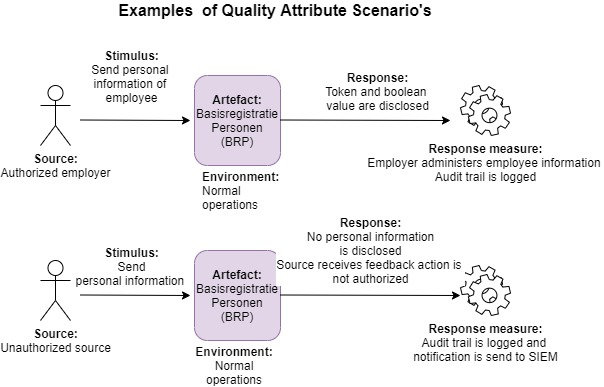
\includegraphics[width=7cm]{QAS-01 ZKP.jpg}\\
\caption{Example of Quality attribute scenario's}
\end{figure}


Zero-knowledge proof itself is a methodology which translates in a variety of technical implementation possibilities. Suitability needs to be assessed per use-case, therefore this research contains an example with high-level scenarios and use-cases depicted in figure \ref{fig:ZKP_usecase}.

This use-case contains three acting parties, namely the employee, employer and tax authorities (Belastingdienst).
Firstly a citizen registers finishes it's registration of personal data at a municipality or non-residents database desk. After this process is finished the citizen receives a BSN, which serves as a UIN throughout all government administrations. The citizen starts working at an employer, fills in his personal information for the wage declaration, including the BSN (2a). The employer is responsible to administer personal information of its employee (2b) and administer and transfer wage declaration to the tax authorities (4). Based on the BSN in the wage declaration, the tax authority checks the personal identity data (5a). \par
In the happy flow, all information off the employee is correct and wage declaration is processed correctly (5b). However, there are practical exceptions, where an employer administers an incorrect BSN or the set of personal information does not match that BSN. In this case, the wage declaration is processed incorrectly. Impact can be another citizen, with the wrongly entered BSN, being taxed for the wage of another citizen. Correcting this mistakes are costly for the government and intense for a citizen who could be negatively impacted because of a higher wage.

\subsection{Use-case 3: application of zero-knowledge proof}
A possible solution would be to let the employer check the correctness of personal information when hiring a citizen. Section \ref{BRP} describes the BRP as the central database of personal identity data of citizens and could be used for this purpose. However, pushing information from the BRP to an employer is not legally allowed. One of the risks could be not acting in good faith which could result in scraping the database to commit fraud or unauthorized usage of personal data mentioned in section \ref{OP}. Zero-knowledge proof could be a pattern to resolve this problem by providing a check if the data the employer receives from an employee matches with a person in the BRP. Ideally, a Zero-knowledge proof will result in not saving personal information in an employer database. However, if this is mandatory by law it needs to been done or law needs to be changed.
\clearpage

\section{Tactics - Quality attribute 'Confidentiality'}
\graphicspath{ {./images/} }
\begin{figure}
\centering
\label{fig:Tactics}
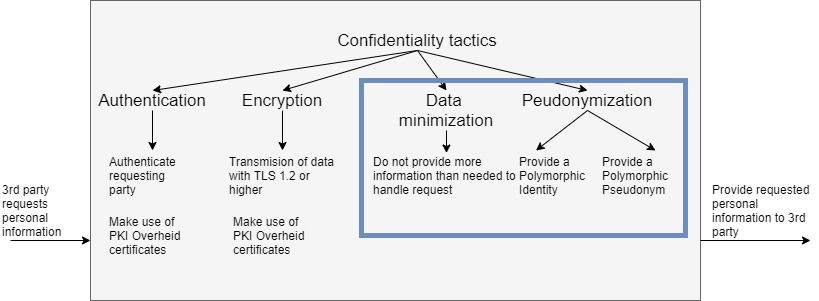
\includegraphics[width=14cm]{Tactics.jpg}\\
\caption{Confidentiality tactics - next section handles examples in blue frame}
\end{figure}

\subsection{Data minimization}
Demanding parties of personal information who are legally permitted to consult the BRP need to search for a person of interest residing on an address. In this case, it can be assumed the personal information has to be shown of only this person of interest. A query which is too broad could give back results of multiple persons. Which could be considered a breach of privacy of those persons. Figure \ref{fig:Adhoc} illustrates a logical view on how a tactic of data minimization could be applied. Firstly, a possible scope of addresses is queried on the Basisadministratie Gebouwen (BAG) \cite{BAG}. The BAG contains almost all addresses within the Dutch territory. Secondly, the correct address is shown and can be selected from this query. If query is a specific statement and returns one result, this result can be selected automatically to support usability. Thirdly, based on the unique address ID from the BAG a list of resident is shown with a minimal set of information to assess if the results contain the person of interest.    
\graphicspath{ {./images/} }
\begin{figure}
\centering
\label{fig:Adhoc}
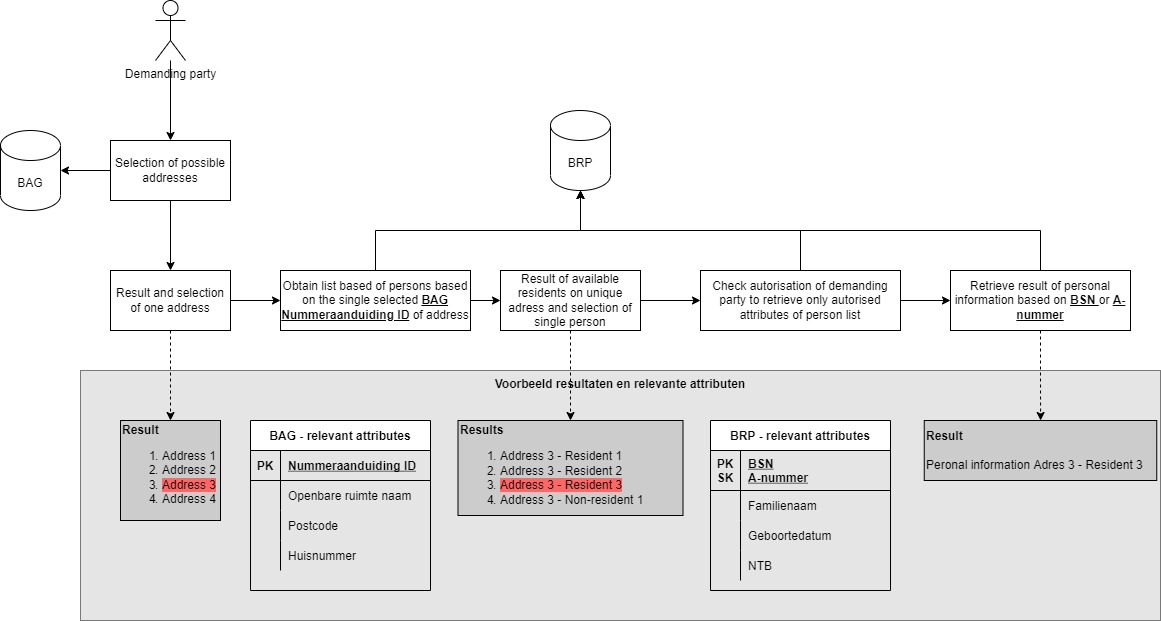
\includegraphics[width=14cm]{Ad-hoc adresvraag dataminimalisatie-EN.jpg}\\
\caption{Logical view - example of data minimization in a process}
\end{figure}

\subsection{Pseudonymization - Polymorphic Identity or Polymorphic Pseudonym}
When it's mandatory to share personal information, because it's for example mandatory by law, it's possible to provide this information as a pseudonym. GDPR \cite{GDPR} defines this method as a possibility to mitigate unwanted disclosure of personal information. 
This technique is already implemented and proven it can work by Erik Verheul \cite{VerheuleID}.

\subsection{Authentication}
A commonly used method for authentication purposes is usage of a certificate. For parties who communicate with on or on behalf of the Dutch government the government issues PKIoverheid (PKIO) certificates. These certificates are used for Authentication, Electronic signatures and encryption. \cite{Logius_PKIO}

\subsection{Encryption - Transfer of data is encrypted with TLS 1.2 or higher}
A broadly implemented standard. The Dutch government has a reference architecture NORA (Nederlandse Overheid Referentie Architecture) \cite{NORA} which states this standard needs to be applied or otherwise explained why it has not been implemented \cite{NORA_PasToeOfLegUit}. On the part of TLS its clear version 1.2 or higher is accepted, but version 1.3 is preferred \cite{NORA_TLS}. 

\section{Trade-offs and concerns}
\todo{Scrapbook, needs refinement}


\begin{tblr}{
 hlines = {white},
 vlines = {white},
 cell{2,3,4,5,6}{1} = {red7}
}
  & Trade-off & Concern & Threats and risk \\
 Maturity & 1 & C-xx, C-xx, C-xx & 3 \\
 Authenticity & 1 & C-xx, C-xx, C-xx & 3 \\
 Accountability & 1 & C-xx, C-xx, C-xx & 3 \\
\end{tblr}

Trade-off snelheid/efficientie. Depends on choosen methodology and algoritm. It's needed to address the needed calculation power (and assumed costs) when selecting algoritms 
\todo{Better describe and support these trade-offs and concerns}



%%% Local Variables:
%%% mode: latex
%%% TeX-master: "../thesis"
%%% End:

\chapter{Related Work}\label{s:related}
\todo{improve and add descriptions (see summary of papers in course 'Knowledge Organization')}

%\todo{
%Describe here scientific papers similar to your experiment, both in terms of %goal and methodology.  One paragraph for each paper (we expect about 5-8 papers %to be discussed). Each paragraph contains: (i) a brief description of the %related paper and (ii) a black-on-white description about how your work differs %from the related paper. You may place this section immediately after the %Background section, if necessary.
%}

\section*{An ISO 25010 Based Quality Model for ERP Systems}
Peters \etal \cite{Peters2020AnI2} provide a guide in implementing ERP systems in higher education institutions (HEI). This research adapts the ISO 25010 standard to specify the quality attributes necessary for selecting an appropriate ERP system for Higher Education institutions. The research describes the application of each of the eight (8) software quality characteristic, also called factors and justifies three (3) new sub-characteristics (or sub-factors) suitable for ERP selection within HEIs. It adds Supportability, Searchability and Archivability as sub-factors. The paper is relevant for this research, because it plots the ISO 25010 on a single type of application. However, this research will not plot every characteristic and sub-characteristic but will point out relevant characteristics. Or Quality Attributes mentioned by Bass \etal \cite{Bass2015SoftwareAI}.

\section*{Consensus Building when Comparing Software Architectures}
Svahnberg and Wohlin \cite{Svahnberg2002ConsensusBW} provide a comparison method on how to produce a comparison of architectures based on quality attributes of the ISO 9126 standard \cite{ISO9126}. The paper explains a method on how to quantify the impact of different architecture types on the assessed quality attributes. It's relevant for my research, because it provides a way to quantify selection of different possible architectures, based on quality attributes. It can be reproduced, based on ISO 25010 and the quality attributes extracted from this research. However, due to restricted amount of time it's not possible to execute the method described. 

\section*{Methodology of Evaluating the Sufficiency of Information for Software Quality Assessment According to ISO 25010}
\todo{add the recap of this paper}
Tetiana Hovorushchenko \cite{Hovorushchenko2018MethodologyOE}

\section*{A guideline for software architecture selection based on ISO 25010 quality related characteristics}
Haoues \etal \cite{Haoues2017AGF} claim it's possible to apply a Software Architecture selection guideline to select an appropriate type of software architecture. They compare relations of the eight (8) main quality characteristics with each other and conclude Functional Suitability, Performance efficiency, Usability and Compatibility are the main drivers to select a type of Software Architecture. The claim is based on extensive literature study and is relevant for this study because it can help predict possible suitable Software Architectures. However, due to restricted amount of time it's not possible to execute the method described. 

\section*{123}
\todo{add one extra relevant paper to commit to minimum of 5 related papers.}
\lipsum[1]
\chapter{Evaluation}\label{s:evaluation}

\section{Design of experiment}
This research puts solutions within the context of a software architecture. It has been done in an inductive research method. The research is based on a theory stating encryption technologies
could be applied more broadly. Theory is gained through literature study and input is gathered via semi-structured interviews. The output of the interviews is coded, resulting in the output for the overview and design section. Validation of output will be done via a focus group working within a relevant project.

\section{Obtained results}

\section{Methodology and biases}

%\todo{
%Discuss the design of your experiments, the results you obtained, and how they
%help in evaluating the claims you made in the introduction. You may also use the
%evaluation results in this section to justify your design choices or assess the
%contributions of different aspects  of your design towards the overall goals.
%}


\chapter{Discussion}\label{s:discussion}
This research leaves implications in current law out of scope, because this in not in scope and not the area of expertise of researcher. Implementations based on this work should be assessed from a legal viewpoint.

\begin{quote}\emph{RQ1: What is the definition of identity fraud and which concrete problems can be identified?}\end{quote} 
In practice, preventing identity fraud is only one of the many business goals to take into account. Also, it could depend on the expertise of the person who will answer this question. Confidentiality is an Architectural Significant Requirement and a Quality attribute of ISO 25010, but not the only Quality attribute that is relevant to consider when designing a system. Also, one could argue it's not quantifiable what kind of real world problems are mitigated with each implemented pattern of tactic in Chapter \ref{s:Implementation}. However, logical reasoning should provide grip evaluating or designing a system. For future work it can be relevant to investigate the impact of mitigating measures and what will drive a citizen to use, or not use, a government system.
\begin{quote}\emph{RQ2: Which requirements are significantly relevant to assess technical suitability and trade offs of these technologies for broader usage within the Dutch government?}\end{quote}
\todo{add a discussion part for this RQ}

\begin{quote}\emph{RQ3: Which architectural tactics and patterns are available and can be used to mitigate identity fraud?}\end{quote}
The selected patterns and tactics are based on the input of consulted experts and interviewees. However, the possible patterns, tactics and matching solutions are inexhaustible and depend on the problem at hand. Two of the concerns not solved in Chapter \ref{s:Implementation} are C-01 "Knowledge of systems an what is legally allowed" and C-02 "Knowledge on encryption and standards is scarce". Both concerns refer to a knowledge problem which could result in problems during implementation or life-cycle. Section \ref{Implications} will state more explicitly  Implications for future research on this topic.

%\todo{
%Here you put your results in context (possibly grouped by research question). %Usually, this section focuses on analyzing the
%implications of the proposed work for current and future research and for %practitioners.
%}

\chapter{Threats To Validity}\label{sec:threats}
Threats to validity of the experiment, according to the classification framework by Wohlin \etal \cite{wohlin12}.
%https://link-springer-com.vu-nl.idm.oclc.org/content/pdf/10.1007%2F978-3-642-29044-2.pdf

\section{Internal Validity}
This research provides a set of architectural significant requirements, tactics and patterns. Combined with an interpretation how to embed these tactics and patterns.
This set can be considered as a starting point and viable selection. However, it will not rule out these tactics and patterns are already in place or other tactics and patterns are better suitable in some situations. If the interviews would be conducted with different subjects in other government or non-governmental organisations it can be assumed the set of variables will be extended or even considered inexhaustible.

\section{External Validity}
This quantitative research is based on a limited amount of interviews. A restricted amount of time and available resources resulted in a limited sample of selected subjects. The outcomes of the interviews can be considered as a pilot. A starting point for further research and actions within the organisation. 
However, the interviewees are experts in the domain of personal identity within the Dutch government. Consulted interdepartmental by other government institutions when it comes to the design and content of the identity system. A source of truth and historical design decisions for different ministries and government departments. The directing architect is involved as peer reviewer for government standards. All subjects have more than 10 years experience at the National office for identity data.  

\section{Construct Validity}
Within this qualitative research semi-structured interviews are used to collect data. Firstly, this method is chosen because the subjects are experts in their fields of expertise, namely personal identity. Limiting them to a questionnaire or structured interview would not provide unexpected and new information or insights in their field of expertise or a correct understanding of the operational problem. Secondly, the use data gathering techniques like unstructured interviews could result in an unlimited stream of information and history. Blandford \etal \cite{Blandford2016QualitativeHR} define that semi-structured interviews “inevitably bring in the interests of the researcher as well as the participant.”. 
\par
It’s needed to acknowledge the bias introduced by the researcher. Blandford \etal \cite{Blandford2016QualitativeHR} define the shaping of data gathering by a researcher as follows: “The researcher is shaping the conversation and the data that is gathered, and the extent of that shaping should be recognized and reported transparently and unapologetically.” The relationship between researcher and subjects is as colleagues within a Dutch government body.

\section{Reliability}
The amount of interviewees and other participants can be considered low. However, the participants are specialists in their field of expertise in maintaining systems of personal data for the Dutch government. Executing this research in other settings, for example commercial parties or a different government body, could deliver different outcomes.
The implementation sections covers one pattern and a set tactics. It can be argued there is a more extensive set of patterns and tactics that can be applied.
\chapter{Conclusion}\label{s:conclusion}
\section{Summary of contributions}
This research defines and quantifies a scope of identity fraud that could impact citizens privacy (1). It demonstrates which Quality Attributes could be considered Architectural Significant Requirements, not only with a scope on Security (2). Applies practical use-cases with technologies to possibly implement and set an example to apply to future processes (3). The solutions in this research are not decomposed in detail, meaning further refinement is needed before building and implementing. However, the decomposition of Architectural Significant Requirements can be used for fundamental blocks designing information systems which exchange personal information. 

\section{Implications for future research}\label{Implications}
On terms of knowledge assurance concerns C-01 and C-02 are describing knowledge of systems and legal applications. These concerns are not resolved in this research but need to be addressed and can be input for further future research on embedding knowledge. Not only looking at the aspects of software systems (for example pattern libraries) but also the organizational aspects of embedding knowledge (for example in-sourcing strategies). 
Also, it needs to be noted not only information technology needs to play a part in solutions. Further research could address other areas of expertise. For example communication and psychology to raise awareness and explain behaviour. Or expertise of law to adapt laws to restrict or oblige certain ways of exchanging personal information. 
Section \ref{s:related} related work shows methods on evaluation and comparison when selecting appropriate software architectures. For future research these methods could be applied on outcomes of this research.

%\todo{
%Briefly summarize your contributions, and share a glimpse of the implications of
%this work for future research.
%}
      
            
% --------------------------------------------------------------
%:                  BACK MATTER: appendices, refs,..
% --------------------------------------------------------------

% the back matter: appendix and references close the thesis


%: ----------------------- bibliography ------------------------

% The section below defines how references are listed and formatted
% The default below is 2 columns, small font, complete author names.
% Entries are also linked back to the page number in the text and to external URL if provided in the BibTex file.

% PhDbiblio-url2 = names small caps, title bold & hyperlinked, link to page 
%\begin{multicols}{2} % \begin{multicols}{ # columns}[ header text][ space]
%\begin{tiny} % tiny(5) < scriptsize(7) < footnotesize(8) < small (9)

\bibliographystyle{Latex/Classes/PhDbiblio-url2} % Title is link if provided
\renewcommand{\bibname}{References} % changes the header; default: Bibliography

\bibliography{references} % adjust this to fit your BibTex file

% this file is called up by thesis.tex
% content in this file will be fed into the main document

%: ----------------------- name of chapter  -------------------------
\appendix 
\chapter{Interviewees} \label{Appendix A} % top level followed by section, subsection 
This section will describe the role of interviewees. Appendix B and C contain a cross-reference with this interviewees. 

\begin{longtblr}[
  caption = {List of interviewees and purpose for consultation},
  label = {tab:interviewees},
]{
  colspec = {|XX[2]|},
  rowhead = 1,
  hlines,
  row{even} = {gray9},
  row{1} = {red7},
} 
Interviewee number and role name & Purpose for consultation\\
 I-01 Stelselspecialist (EN: System specialist)   &  \\
 I-02 Informatie analist (EN: Information Analyst) &  \\
 I-03 Regie architect (EN: directing architect) & \\
 I-04 Adviseur Digitalisering (EN: Advisor digitization) &\\
 I-05 Chief Information Security Officer & Consulted as a source for relevant standards and techniques (patterns and tactics)\\
\end{longtblr}

\chapter{Business goals} \label{Appendix B} % top level followed by section, subsection
This section will cover output of interviews and contains a brief overview of business goals. Raw output of interviews and code document (as far as NDA allows \todo{check NDA within RvIG}) are added in the replication package of this research.


\begin{longtblr}[
  caption = {List of Business Goals},
  label = {tab:business_goals},
]{
  colspec = {|XX[3]|},
  rowhead = 1,
  hlines,
  row{even} = {gray9},
  row{1} = {red7},
} 
Business goal number and name & Description & Addressed by\\
 BG-01 Explainable solutions   &   Communicate simple how technology works to raise awareness and support. Also, provide more detailed scientific information for experts to contribute as a community. &  I-03\\
 BG-02 (Re-)Use of available standards and patterns &  Reusage of standards and patterns is a goal to keep systems maintainable and portable. It also helps in building a knowledge base that can be applied on multiple products & I-03\\
 BG-03 Apply a 'Zero knowledge proof' or minimalize data exchange & "Minimalize the amount of data transfered. If data is not available it can not be stolen in case of for example a databreach.GDPR states a minimalization of data in Article 5. Only provide information that is needed for the initial purpose.Ultimately, it's desired to only acknowledge if the provided personal information is correct, without providing the information itself. Also known as a 'Zero knowledge proof'." & I-01 and I-03 \\
BG-04 Maintain a unique identity of a person within a whole chain & Big advantage of maintaining a unique identity (number) of a person within a whole chain of government body, prevent rework and multiple different ways of administering a single person. & I-01 and I-02 \\
 BG-05 Provide ease of use and uniform (self)service solutions to a citizen, together with chain partners &  Services provided to citizens (both residential and non-residential) are uniformly provided by each government body. Currently, this is mainly provided by having a DigiD that is on itself based on the unique BSN of a citizen. & I-01 and I-02\\
 BG-06 Provide identity data outside government organisations, while preserving citizens privacy & Usage of identity information of the 'Basisregistratie personen (BRP)' is now limited to a small selection of government and non-government organizations. It can be assumed more non-government organizations will need to verify an identity, while the identity information itself is not provided to that company. & I-04 \\
\end{longtblr}

\chapter{Concerns} \label{Appendix C}
This section will cover output of interviews and contains a brief overview of concerns. Raw output of interviews and code document are added in the replication package.

\begin{longtblr}[
  caption = {List of Concerns},
  label = {tab:concerns},
]{
  colspec = {|XX[3]|},
  rowhead = 1,
  hlines,
  row{even} = {gray9},
  row{1} = {red7},
} 
Concern number and name & Description & Addressed by\\
C-01 Knowledge of systems and what is legally allowed    &   Area of expertise within the identity domain is complex and system specialists (NL: Stelselspecialisten) and other specialists are a rare resource. History of law and systems is implicit knowledge or hard to find in documentation. When designing new systems it's needed to comprehend the domain and its internal and external influences. & I-03\\
 C-02 Knowledge of encryption and standards is scarce &  Area of expertise within technological field of encryption standards is complex and specialists are a rare resource. & I-03\\
 C-03 Secure transfer of personal data  &  Transfer of personal data is necessary by law, but needs to be done in a safe and secure way. & I-03 \\
C-04 Uniqueness of key, but vulnerable because of process
& One BSN can be assigned to multiple persons or multiple BSN can be assigned to one person. These incidents can happen and are mitigated by processes within RvIG and can be reported by the citizen at the Meldpunt Fouten in Overheidsregistraties since January 2021. An suggested alternative could be the A-nummer, which' uniqueness is guaranteed in by referential intergrety of the database. & I-01 and I-02\\
C-05 Uniqueness of key, but vulnerable because of misuse & BSN as a UIN is broadly used within government bodies and commercial parties. It's not possible to control all applications of BSN, while this UIN is important to identify a unique person. Therefore, it's a vulnerable object within identity data. & I-01 \\
C-06 Identity misuse & Is the person using the identity data the person that belongs to that specific identity & I-02\\
C-07 Citizen sees the government in a broader perspective than the government itself & Usage of BSN is positioned as a number that can only be used by authorized organization, allowed by law. While a citizen sees the (responsibilities of the) government bigger than the government itself. Not allowing organizations to access data of the citizen, while the citizen himself expects the organization to access that data could have a mismatch in service expectations. & I-01\\
C-08 BSN not available, while rights may apply & A person lives and/or works in The Netherlands, but does not have a BSN. Or a person lives in a foreign country, but has rights in The Netherlands (like a pension). In that circumstances there are rights, but no identification number & I-01\\
C-09 As a government it’s needed to take in account all possible exceptions & A commercial organization could argue a data quality of for example 98\% is almost perfect and enough to maintain a high level of service. A government body needs to take in account that 2\% of it's population is a few 100.000 people that could have not overseen troubles in their contact with government and non-government organizations that for example authenticate that person and base decisions on the provided data. & I-01\\
C-10 Recognizing and authentication of a person is linked intensively with the BSN & There are processes relying on solely a person having a BSN number, while it could be possible to have rights without having a BSN. Also, authenticating a person is relying a lot on having the correct BSN, while it was not the purpose of BSN to authenticate a person. & I-01 \\
C-11 Laws and practical implementations focus on BSN as a primary key that needs to be used & While the practical implementation could be done without BSN, sometimes it's designated by law this primary key is leading and needs to be used & I-04 \\
C-12 Non-government sectors need to exchange information on citizens & Non-government sectors, like banks, insurance companies or mortgage lenders, need to exchange information of citizens with other non-government organizations. They need to verify an identity before exchanging information, while preserving privacy could make this more complex. Administering signals of fraud or creditworthiness wrongly could impact a citizen negatively. & I-04

\end{longtblr}


% ---------------------------------------------------------------------------
%: ----------------------- end of thesis sub-document ------------------------
% ---------------------------------------------------------------------------



%\end{tiny}
%\end{multicols}



% --------------------------------------------------------------
% Various bibliography styles exit. Replace above style as desired.

% in-text refs: (1) (1; 2)
% ref list: alphabetical; author(s) in small caps; initials last name; page(s)
%\bibliographystyle{Latex/Classes/PhDbiblio-case} % title forced lower case
%\bibliographystyle{Latex/Classes/PhDbiblio-bold} % title as in bibtex but bold
%\bibliographystyle{Latex/Classes/PhDbiblio-url} % bold + www link if provided

%\bibliographystyle{Latex/Classes/jmb} % calls style file jmb.bst
% in-text refs: author (year) without brackets
% ref list: alphabetical; author(s) in normal font; last name, initials; page(s)

%\bibliographystyle{plainnat} % calls style file plainnat.bst
% in-text refs: author (year) without brackets
% (this works with package natbib)


% --------------------------------------------------------------

% according to Dresden med fac summary has to be at the end
%
% Thesis Abstract -----------------------------------------------------


%\begin{abstractslong}    %uncommenting this line, gives a different abstract heading
\begin{abstracts}        %this creates the heading for the abstract page

\noindent \textit{Context}. 
Privacy of citizens is protected by law. However, leakage of citizens' data occurs more often with possible impact on the live of these citizens.

\noindent \textit{Goal}. 
Goal of this research is to provide an overview of the domain of identity theft and to provide a definition of concrete problems together with possible solutions.

\noindent \textit{Method}. 
Research experiment has been executed based on literature study and semi-structured interviews with experts in the field of identity data within the government. 
Using coding to extract information from the semi-structured interviews.

\noindent \textit{Results}. 
The extracted Business Goals and Concerns resulted in Architectural Significant requirements which lead to possible privacy mitigating solutions as examples for implementation.

\noindent \textit{Conclusions}. 
Identity theft is a broad domain and to solve problems it needs scoping. In the solution part Architectural Significant Requirements can facilitate in selecting an appropriate solution.

\end{abstracts}
%\end{abstractlongs}


% ---------------------------------------------------------------------- 


%: Declaration of originality
%\include{8_backmatter/declaration}



\end{document}
